% Please do not change the document class
\documentclass{scrartcl}

% Please do not change these packages
\usepackage[hidelinks]{hyperref}
\usepackage[none]{hyphenat}
\usepackage{setspace}
\usepackage{graphicx}
\doublespace

% You may add additional packages here
\usepackage{amsmath}

% Please include a clear, concise, and descriptive title
\title{How the use of Personas in Agile may Allow Game Developers to Construct more Focused and Prioritised User Stories}

% Please do not change the subtitle
\subtitle{COMP150 - Agile Essay}

% Please put your student number in the author field
\author{1507290}

\begin{document}

\maketitle

\abstract{Agile agile agile abstract}

\section{Introduction}
The Agile methodology itself does not directly address usability. The Agile Manifesto~\cite{} is focused on the development process. Despite some conflicts in principles, interest in incoorporating user centred design (UCD) methods into Agile is growing~\cite{haikara:extending}. One such UCD tool which has been integrated into some Agile methods is the use of Personas~\cite{caballero:persona}. Personas are a set of fictional characters created to be archetypal of the different groups of intended users. Their primary purpose is to solidify the concept of the end user to help designers and developers more effectively understand the product's intended users. 
Games are solely about the user's experience of the game, so an understanding of the user is especially important. This essay will explore how the use of personas and agile in games development could help create a game that provides the user with a better experience, as well as helping user stories be constructed and prioritised more effectively.

%Personas help designers and developers more effectively capture the needs of their intended product users, as well as being a tool to aid communication. Personas are a fictitious character that is created as an archetype of a group of intended users, usually based on empirical data \cite{}. In agile, they are then usually placed on the task board or in a notable place in the team's working environment \cite{}. A persona is less abstract than a vague idea of the target market's characteristics, and can help developers and designers more carefully consider how they would use the product and what their goals are. This is especially useful in situations where the success of the product heavily lies on the end user's experience \cite{}. Game development is one such field. Consequently, the integration of personas into the Agile process in games development teams may help game developers create more effective user stories that encourage them to keep the actions of those who are playing the game in mind.

\section{The Benefits of using Personas}
Personas can help designers, developers and testers more effectively capture the needs of their intended product users, as well as being a tool to aid communication. Personas usually contain information about the user such as name, age, occupation, a photo, and the goals of that Persona when using the product. In agile, they are usually placed on the task board or in a notable place in the team's working environment \cite{}. Persona's can help developers and designers more carefully consider how users would use the product and what their goals are, since they are concretely defined rather than abstract sections of the target market. Understanding how the user will experience the product is especially important in a field such as games, which is all about the user's enjoyment. \cite{}.

Personas can also be used as an effective communication tool between team members and departments~\cite{}.

%The use of personas throughout the design and development process ensures that end users are kept in mind throughout. It also serves to solidify the target users, instead of them being an abstract concept. This is because personas should be developed as a result of research. Understanding how the user will experience the product is especially important in a field such as games, which is all about the users enjoyment.

\section{Integrating Personas into Agile}
Some elements of Personas conflict with elements of the Agile manifesto, whilst some parts of their philosophies are similar~\cite{haikara:extending, chaimberlain:framework}. The Persona method in UCD usually involves researching the users and creating the personas before any development begins, whereas Agile discourages this practice~\cite{chaimberlain:framework}. In order to make personas compatible with Agile, they could be made to be iterative, as is demonstrated with `Extreme Personas'~\cite{wolkerstorfer:probing}. This way, the persona's profile would be reviewed and developed alongside the project as requirements change and new information about the users surface. The personas could be reviewed at the end of each sprint, alongside user stories.


%Developing personas alongside user stories may help the user stories be more user based and informed.

\section{How can personas be used in game development?}
It is difficult to focus user stories on users in game development, as all of the users are players. Using personas could provide a way to target the user stories to specific types of user. The priority of user stories could then be determined using the personas' goals and personalities as a guide~\cite{microsoft thing}. 
Another approach to tying personas to user stories is to create persona driven user stories~\cite{winter:vision}; that is, user stories that specifically refer to a single persona. For game development, the goals of the Persona will be of particular importance; they can define why the user is playing the game and what they want to achieve in the game. 
\begin{figure}[h]
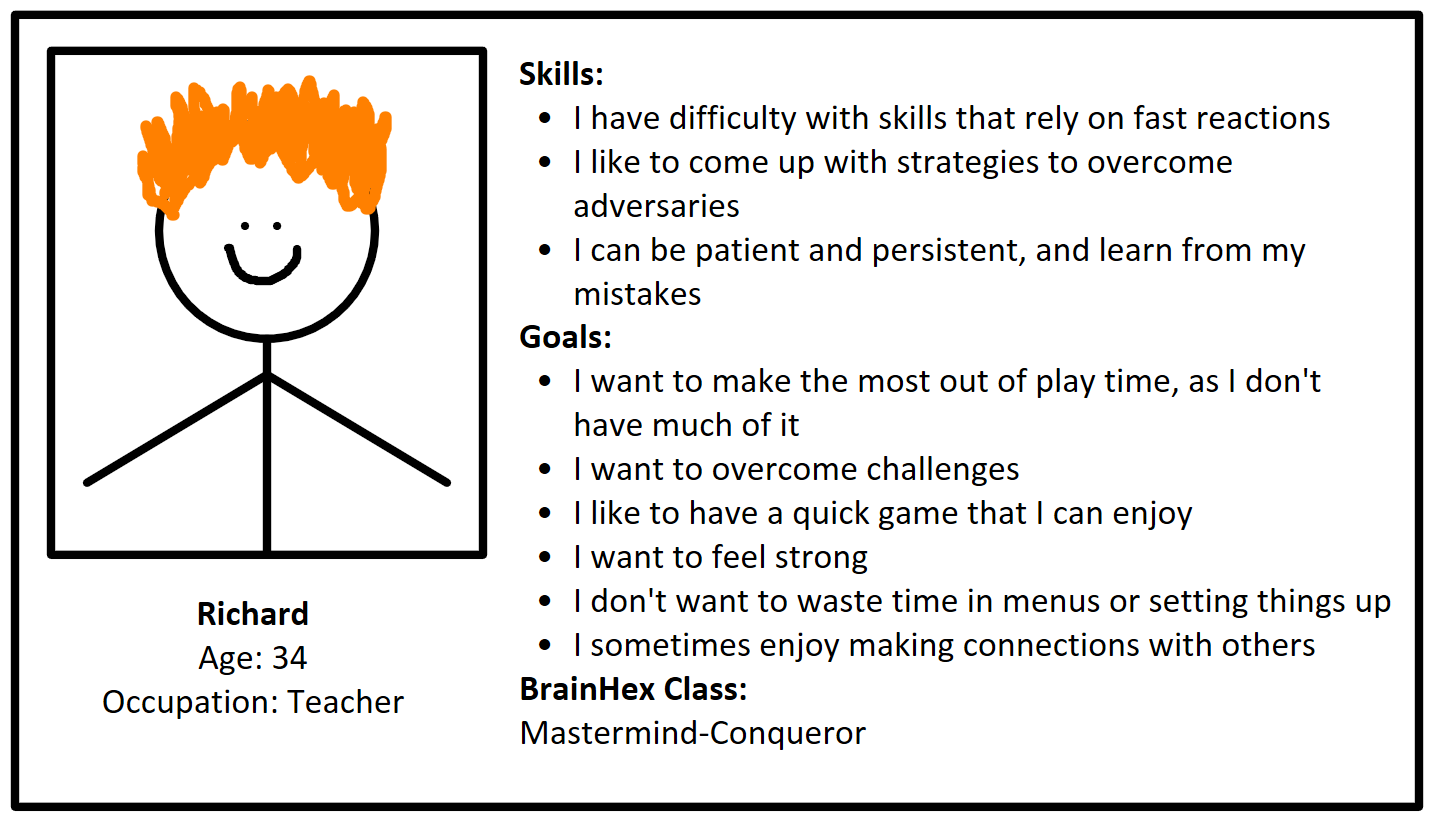
\includegraphics[width=\textwidth]{example.png}
\caption{An example of a Persona for game development}
\label{fig:persona_example}
\end{figure} 
Additionally, a persona for game development could include the player's gamer type according to taxonomies such as Brainhex~\cite{nacke:brainhex}, the Bartle test\cite{bartle:mud}, or Yee's taxonomy\cite{yee:online}.  An example of the information a game development persona could include is illustrated in Figure~\ref{fig:persona_example}. 


%The use of personas in game development, therefore, may help developers focus on who is going to be playing their game and better design for them.


\section{Conclusion}
Bye.

\bibliographystyle{ieeetran}
\bibliography{comp150_agile}

\end{document}
